\section{Langkah-Langkah Percobaan}
\subsection{Crimping}
Percobaan ini diawali dengan melakukan crimping pada kabel UTP berdasarkan urutan warna seperti standar nasional T568A dengan pemasangannya menggunakan Straight-through. Bahan-bahan yg digunakan meliputi :
\begin{enumerate}
    \item Kabel UTP
    \item RJ45
    \item Tang crimping 
    \item LAN tester 
\end{enumerate}
berikut proses melakukan crimping untuk konfigurasi kabel LAN. 
\begin{figure}[H]
    \centering
    \begin{subfigure}[b]{0.3\linewidth}
      \centering
      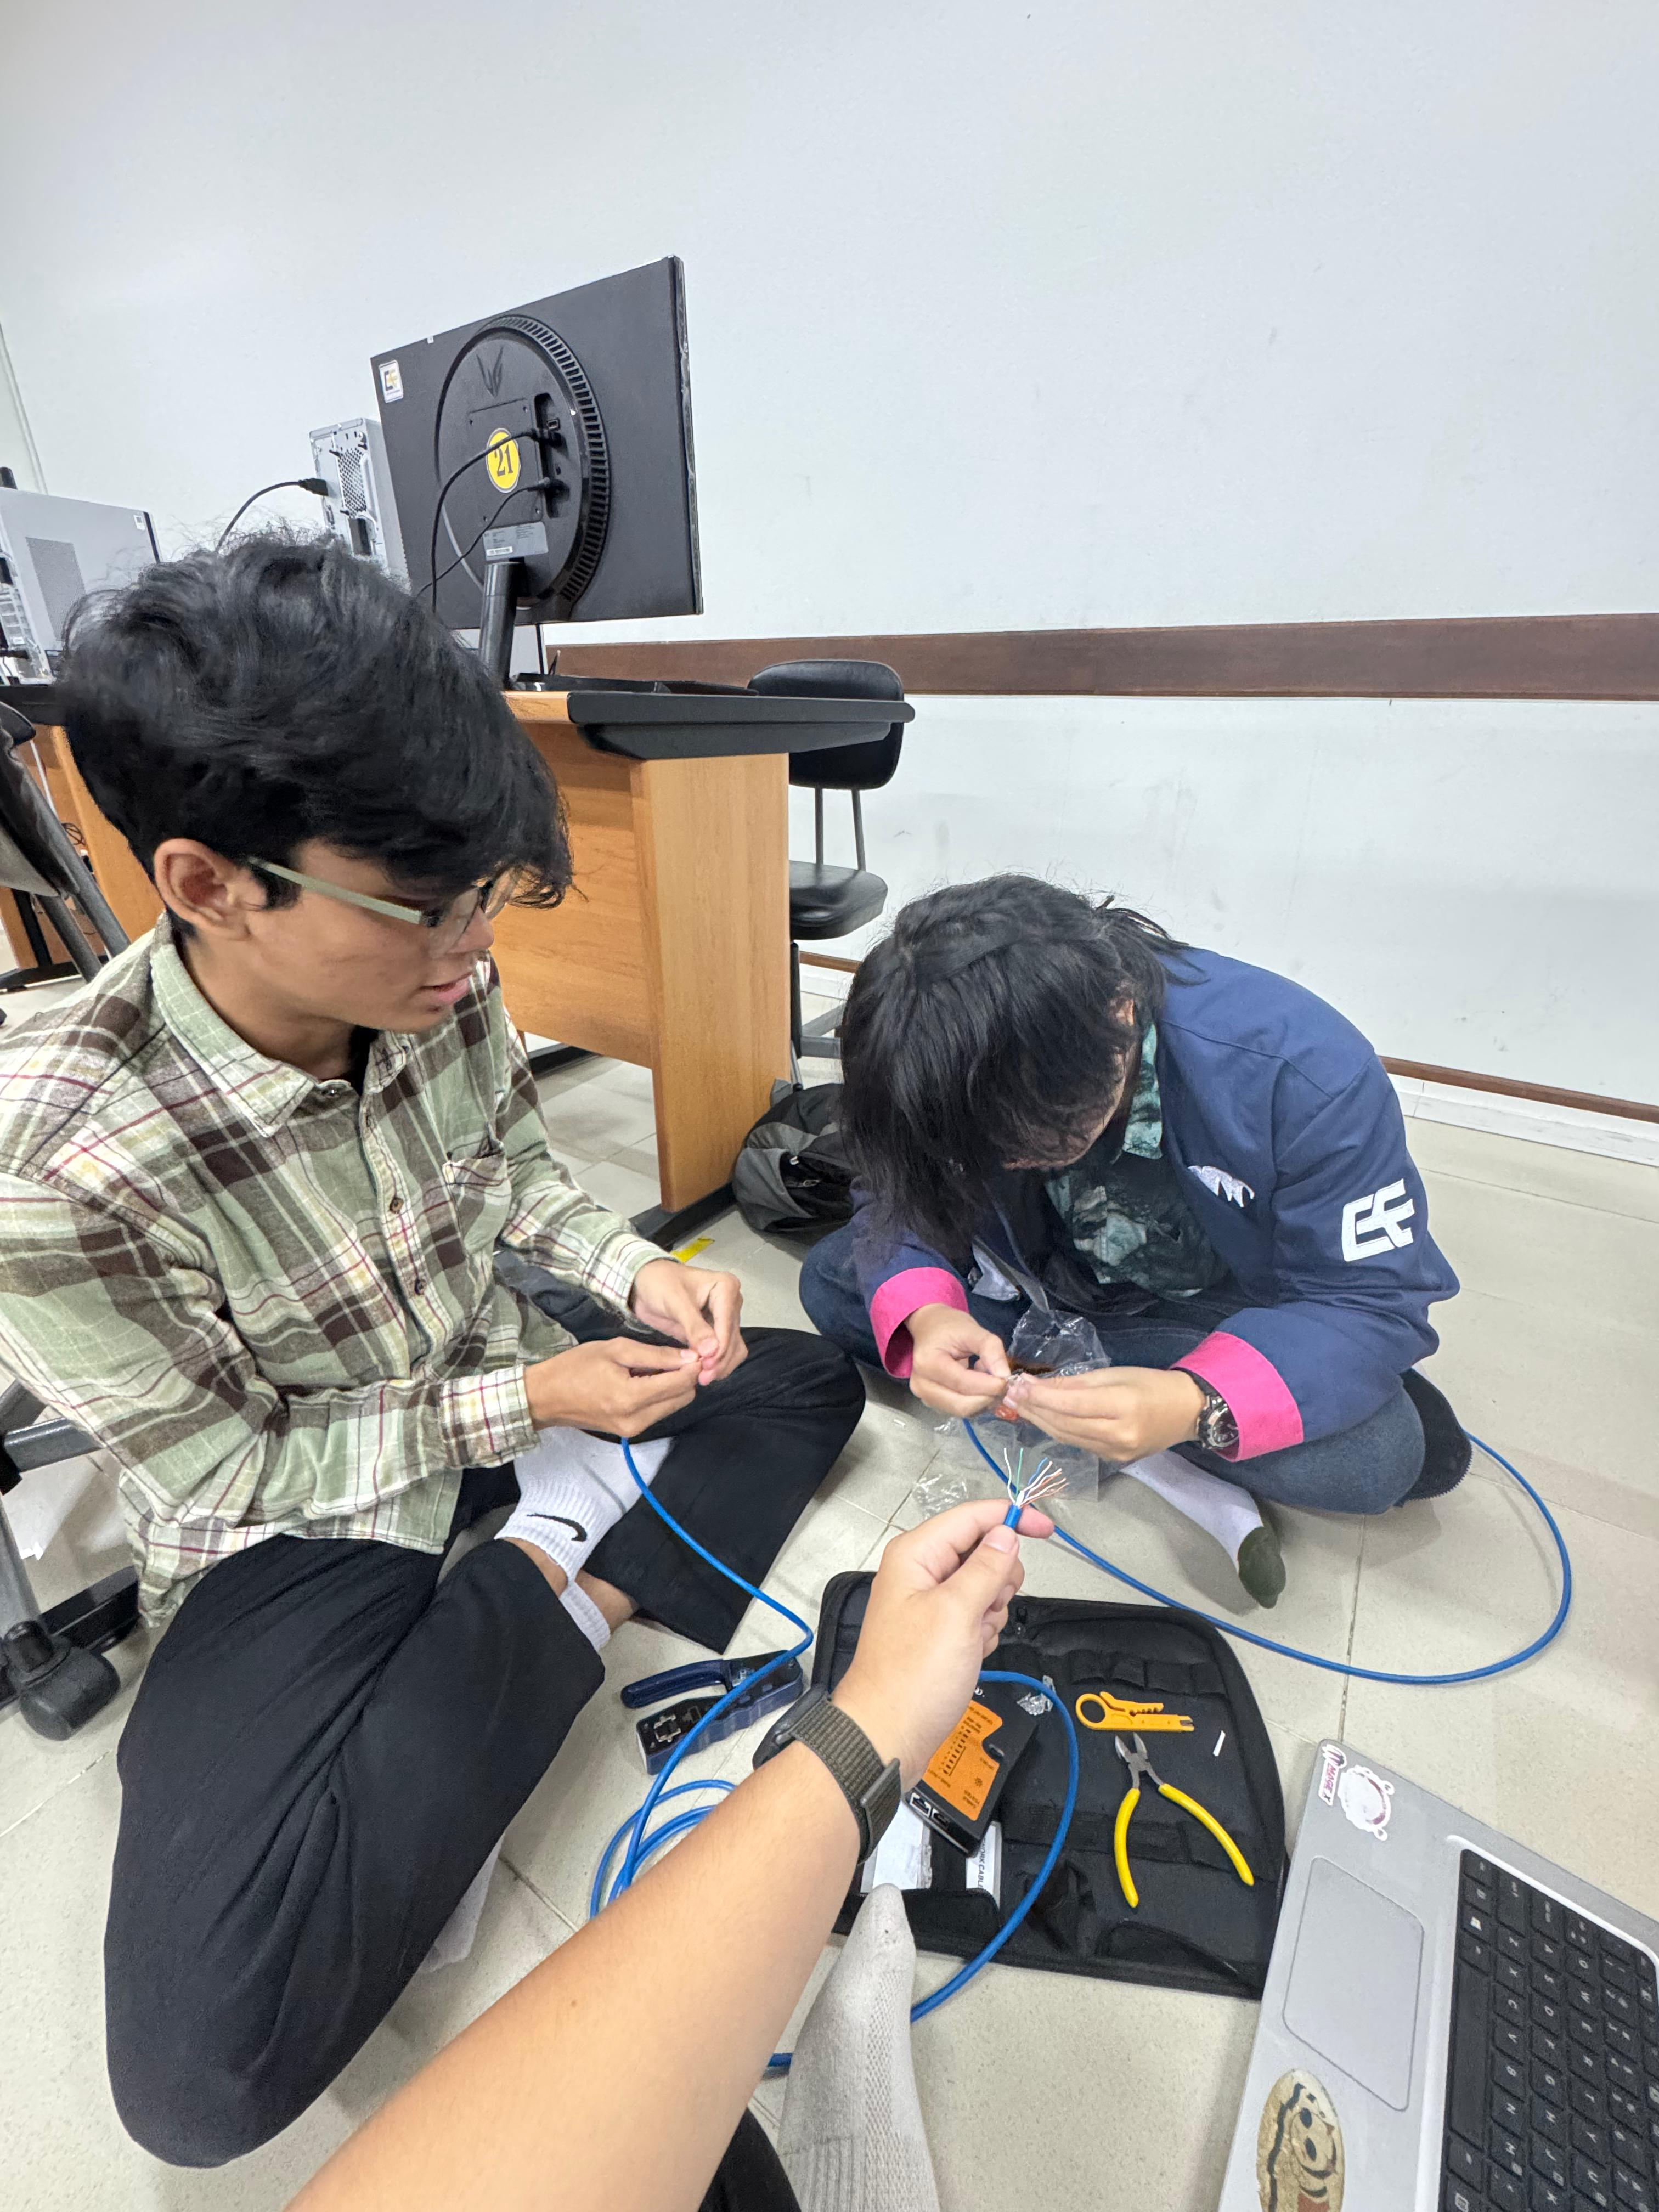
\includegraphics[width=\linewidth]{image/crimping1.jpg}
      \caption{mengurutkan warna kabel T568A}
    \end{subfigure}
    \hspace{1cm}
    \begin{subfigure}[b]{0.3\linewidth}
      \centering
      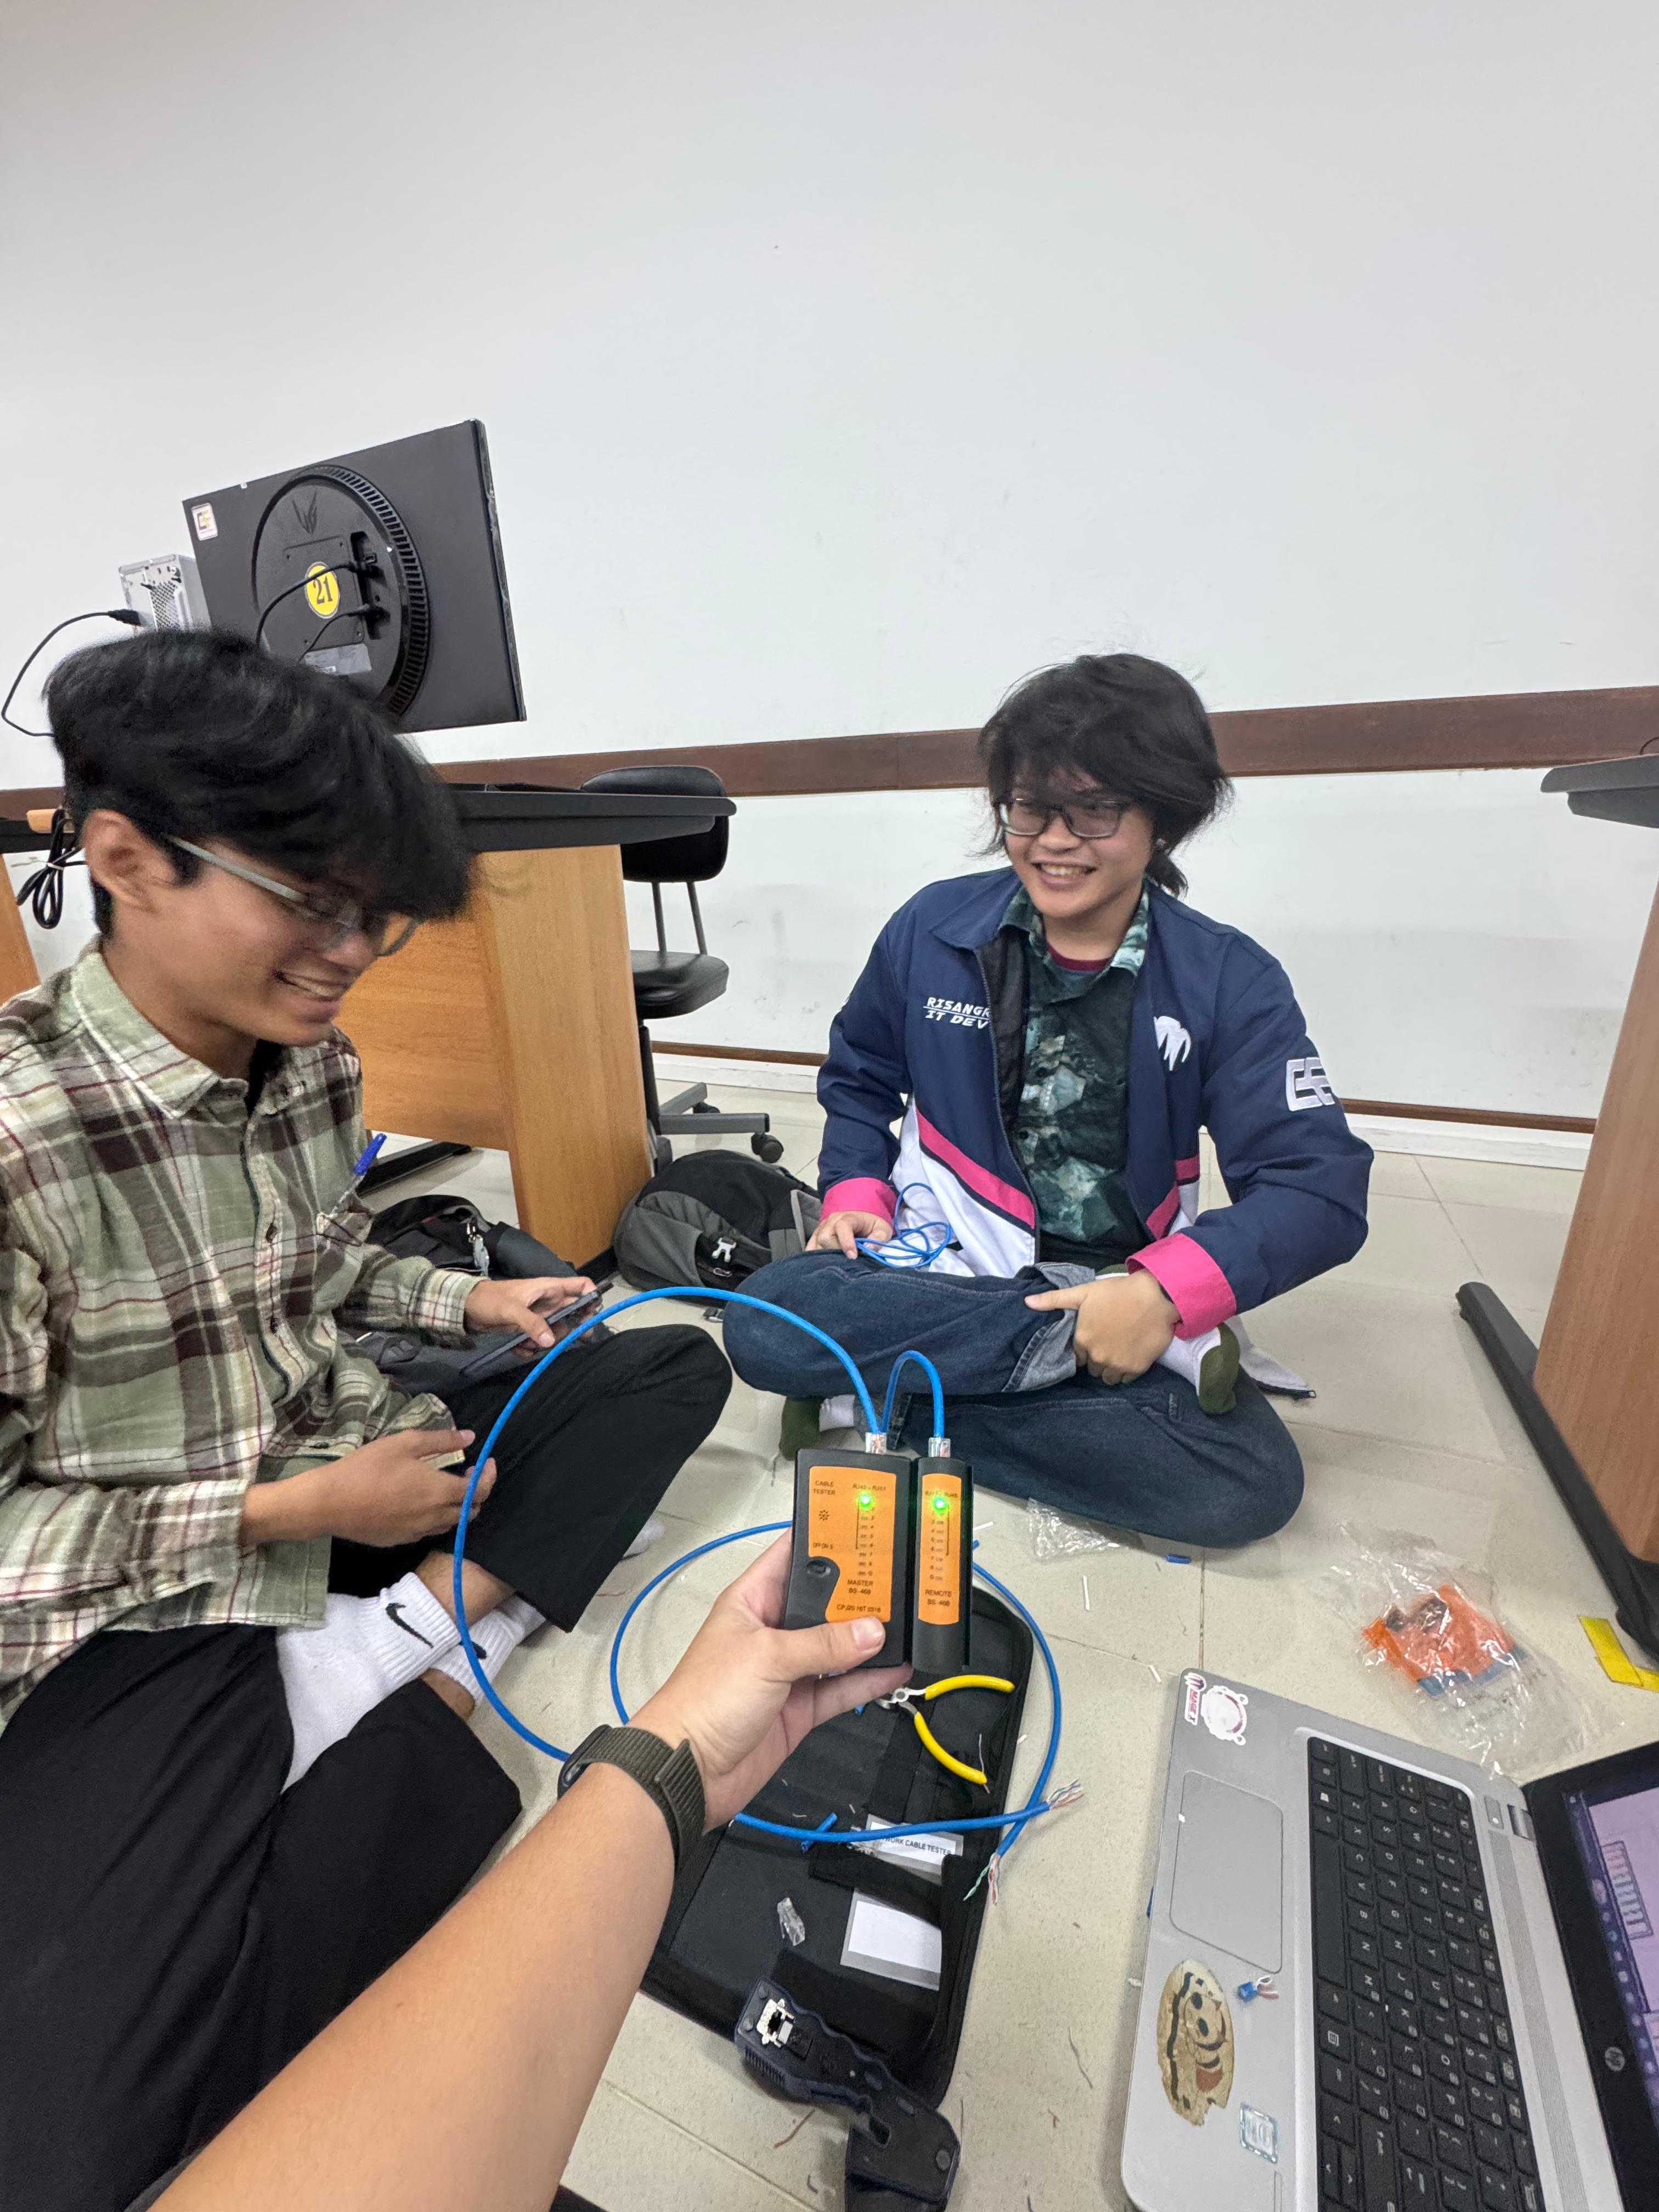
\includegraphics[width=\linewidth]{image/crimping2.jpg}
      \caption{mengecek kabel hasil crimping}
    \end{subfigure}
    \caption{Crimping ini dilakukan dengan metode Straight-Through yang digunakan untuk menyambungkan dua tipe perangkat berbeda yang tersambung ke jaringan.}
\end{figure}

\subsection{Routing Statis}
Routing pada percobaan ini menggunakan 2 cara yaitu statis dan dinamis. Routing ini menggunakan 2 router mikrotik yang akan menyambungkan 2 laptop. Berikut langkah-langkah routing secara statis. \\ 
1. Reset konfigurasi untuk kedua router, lalu login ke router mikrotik dengan menggunakan software Winbox.\\
2. Konfigurasi IP Address pada Ether1 menggunakan prefix /30, 10.10.10.1 untuk router 1 dan 10.10.10.2 untuk router 2. Lalu konfigurasi IP Address untuk jaringan LAN pada Ether2 untuk menghubungkan laptop dengan router, gunakan prefix /27 dan untuk IP Address untuk router 1 192.168.10.1/27 dan router 2 192.168.20.1/27. \\
3. Menambahkan route secara manual. pada Ether2, router 1 Dst.address diisi dengan alamat network router 2 dan sebaliknya dengan alamat yaitu 192.168.20.0/27 dan 192.168.10.0/27. Pada Ether1, konfigurasi gateway masing-masing router dengan alamat 10.10.10.1 dan 10.10.10.2. \\
\begin{figure}[H]
    \centering
    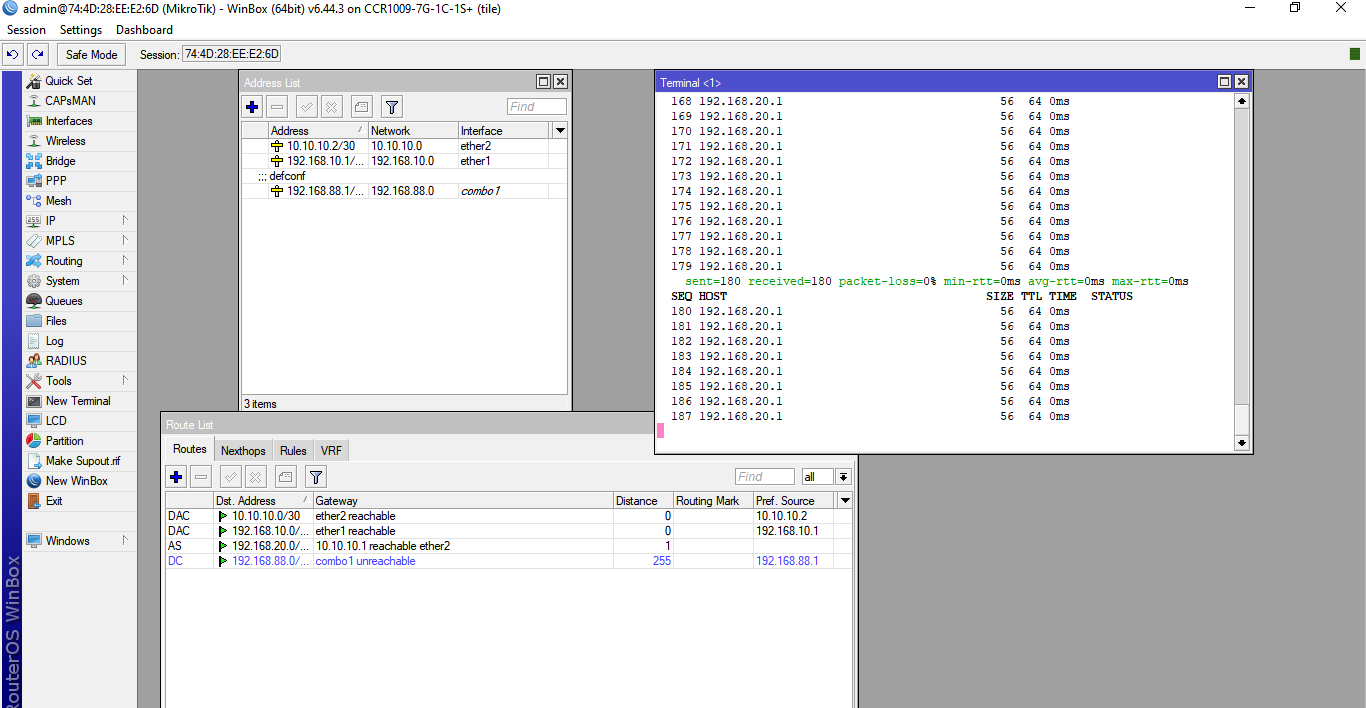
\includegraphics[width=0.65\linewidth]{image/routing1.png}
    \label{fig:inirujukan}
    \caption{Berikut langkah-langkah pada poin 2 dan 3 serta hasil uji ping pada Winbox}
\end{figure}
4. Karena menggunakan IP statis, tambah IP Address secara manual ke interface di kedua laptop lewat setting windows, IP dan gateway harus sesuai dengan Ether2. Lalu uji tes ping ke masing-masing laptop.
\begin{figure}[H]
    \centering
    \begin{subfigure}[b]{0.3\linewidth}
      \centering
      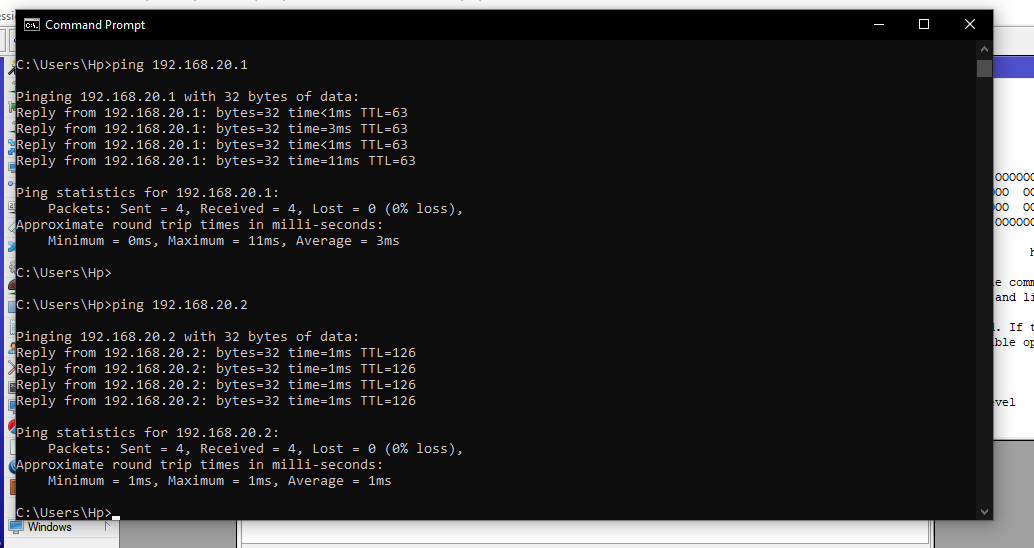
\includegraphics[width=\linewidth]{image/routing2.png}
      \caption{laptop 1 ke laptop 2}
    \end{subfigure}
    \hspace{1cm}
    \begin{subfigure}[b]{0.3\linewidth}
      \centering
      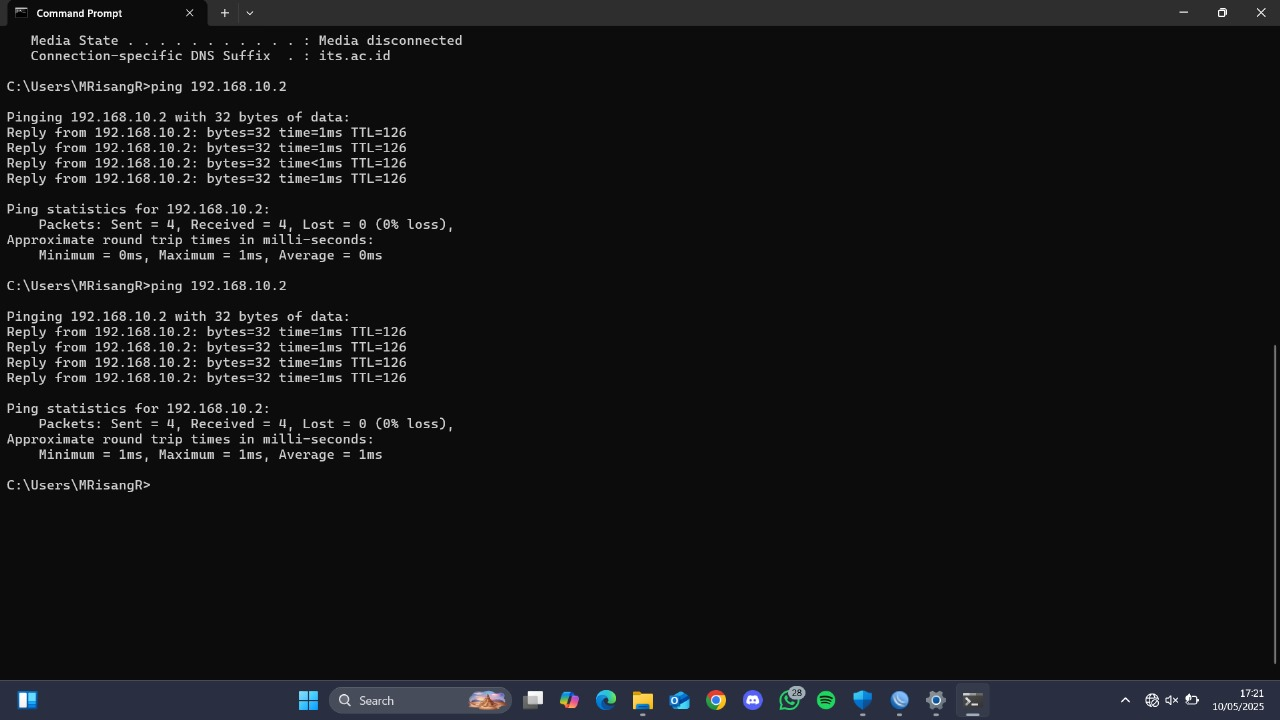
\includegraphics[width=\linewidth]{image/routing3.jpg}
      \caption{laptop 2 ke laptop 1}
    \end{subfigure}
    \caption{Hasil tes ping untuk masing-masing laptop menggunakan cmd}
\end{figure}

\subsection{Routing Dinamis}
Routing dinamis adalah mekanisme routing di jaringan komputer yang memungkinkan router untuk secara otomatis membuat dan mengupdate tabel routing mereka berdasarkan informasi yang diterima dari router lain. Berikut langkah-langkah roting secara dinamis. \\
1. Reset konfigurasi kedua router, lalu login ke router mikrotik dengan Winbox. \\
2. Aktifkan Routing RIP Package. Konfigurasi IP Address pada Ether1 Tambahkan IP address pada ether1 yang digunakan sebagai jalur antar-router. Karena hanya ada dua perangkat yang terhubung menggunakan prefix /30, 10.10.10.1/30 dan 10.10.10.2/30. Konfigurasi IP Address untuk Jaringan LAN ether 2 Tambahkan IP address pada ether 2 yang digunakan untuk menghubungkan Laptop dengan Router menggunakan prefix /27, 192.168.10.1/27 dan 192.168.20.1/27. \\
3. Konfigurasi DHCP server dan sesuaikan interface ethernet menjadi 2. \\
4. Konfigurasi routing dinamis menggunakan RIP. untuk interface gunakan ether all, setting revice menjadi V1-2, Send menjadi V-2, dan authentification menjadi none. Tambahkan network pada RIP dan masukkan IP network yang ada di router sendiri. Tambahkan gateway jaringan dengan alamat gateway komputer tujuan. \\ 
\begin{figure}[H]
    \centering
    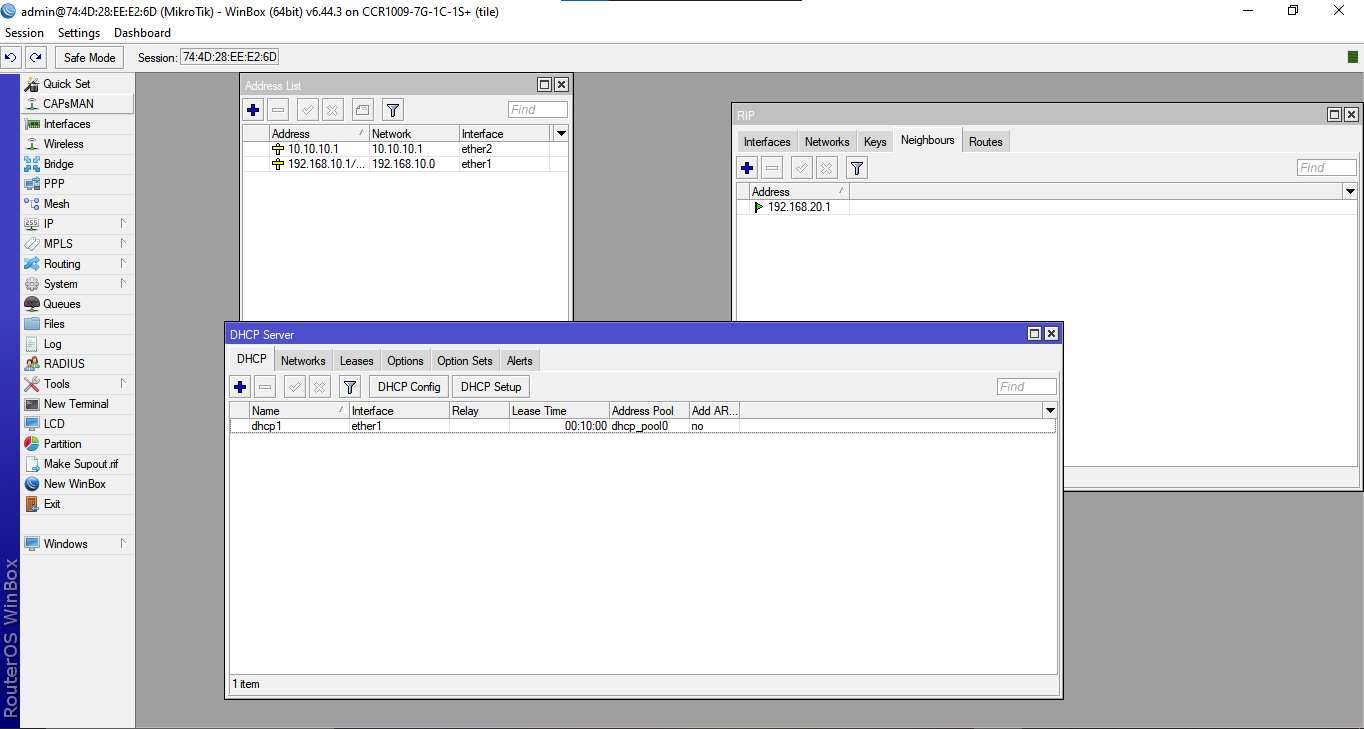
\includegraphics[width=0.65\linewidth]{image/routing4.png}
    \label{fig:inirujukan}
    \caption{Berikut langkah-langkah pada poin 2-4}
\end{figure}
5. Lakukan uji tes ping antara 2 laptop 
\begin{figure}[H]
    \centering
    \begin{subfigure}[b]{0.3\linewidth}
      \centering
      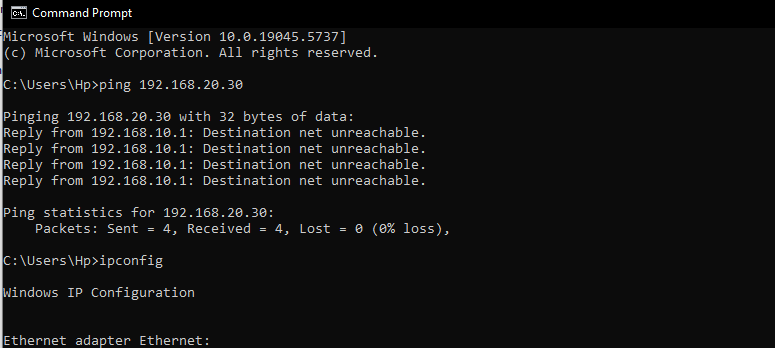
\includegraphics[width=\linewidth]{image/routing5.png}
      \caption{laptop 1 ke laptop 2}
    \end{subfigure}
    \hspace{1cm}
    \begin{subfigure}[b]{0.3\linewidth}
      \centering
      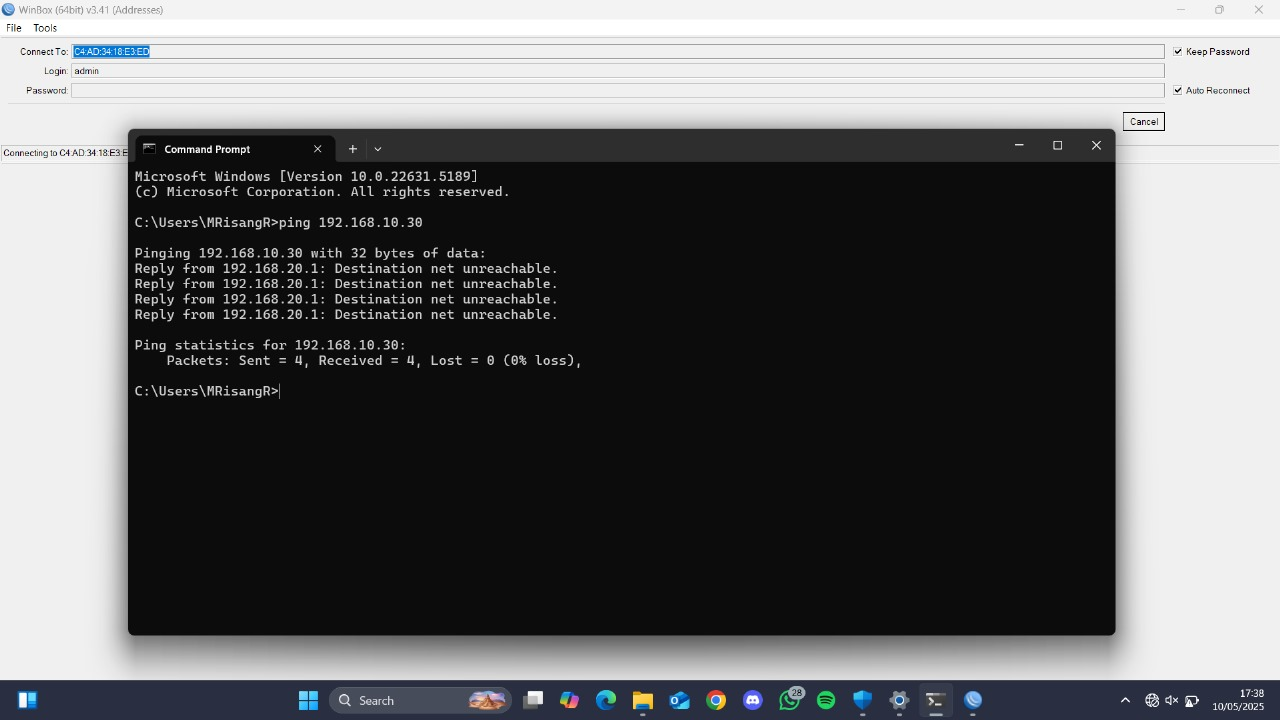
\includegraphics[width=\linewidth]{image/routing6.jpg}
      \caption{laptop 2 ke laptop 1}
    \end{subfigure}
    \caption{Hasil tes ping unreachable untuk masing-masing laptop menggunakan cmd}
\end{figure}

\section{Analisis Hasil Percobaan}
Pada praktikum Modul 1, praktikan melakukan kegiatan berupa crimping kabel UTP dengan konektor RJ45 dan melakukan routing jaringan IPv4 untuk menguji konektivitas antar perangkat. Tujuan percobaan ini adalah agar praktikan mampu memahami secara praktis proses pembuatan kabel jaringan serta pengaturan alamat IP dan routing pada jaringan komputer. 
\subsection{Perbandingan Hasil Percobaan dengan Teori}
Berdasarkan teori, penyusunan kabel UTP dengan standar T568A akan menghasilkan koneksi yang berbeda, Straight-Through untuk perangkat berbeda. Hasil yang diperoleh Kabel yang disusun dengan urutan warna yang benar dan dikrimping dengan benar dapat mengalirkan data dan menunjukkan lampu indikator aktif saat diuji menggunakan LAN tester. \\
Routing IP secara teori membutuhkan pemberian alamat IP yang tepat dan pengaturan rute secara statis atau dinamis agar paket data dapat mengalir dari satu jaringan ke jaringan lain. Dalam percobaan, konfigurasi alamat IP dan pengujian konektivitas melalui perintah ping menunjukkan bahwa routing berhasil dilakukan, terutama pada konfigurasi routing statis.
\subsection{Faktor yang Mempengaruhi Hasil}
Pada saat proses crimping, urutan warna kabel yang sering terbalik saat proses memasukannya ke dalam RJ45 dan pin yang tidak sepenuhnya menempel. Hal tersebut menyebabkan koneksi gagal dan lampu indikator pada LAN tester tidak menyala sepenuhnya. \\
Jangka waktu yang pendek, karena proses crimping yang banyak masalah dan memakan waktu praktikum. Jadi, untuk proses routing tidak sepenuhnya terselesaikan.

\section{Hasil Tugas Modul}
\begin{figure}[H]
    \centering
    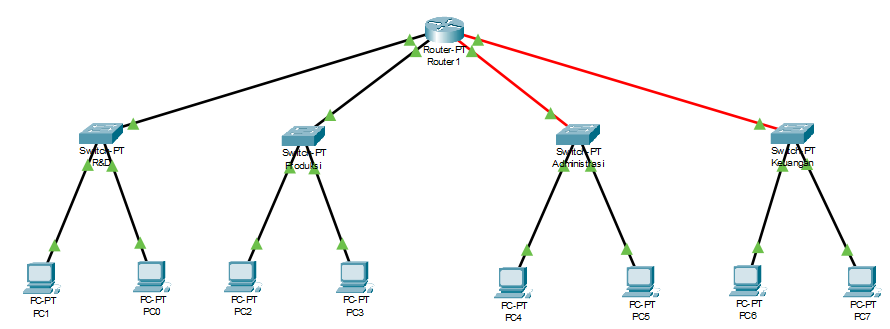
\includegraphics[width=0.65\linewidth]{image/topologi.png}
    \label{fig:inirujukan}
    \caption{Hasil topologi}
\end{figure}
Hasil tersebut merupakan topologi jaringan dari 4 departemen yang dihubungkan melalui 1 router. Konfigurasi pada IP dan gateway untuk masing-masing departemen sama dengan tabel pada tugas pendahuluan. Berikut ini merupakan uji ping antar departemen. 
\begin{figure}[H]
    \centering
    \begin{subfigure}[b]{0.3\linewidth}
      \centering
      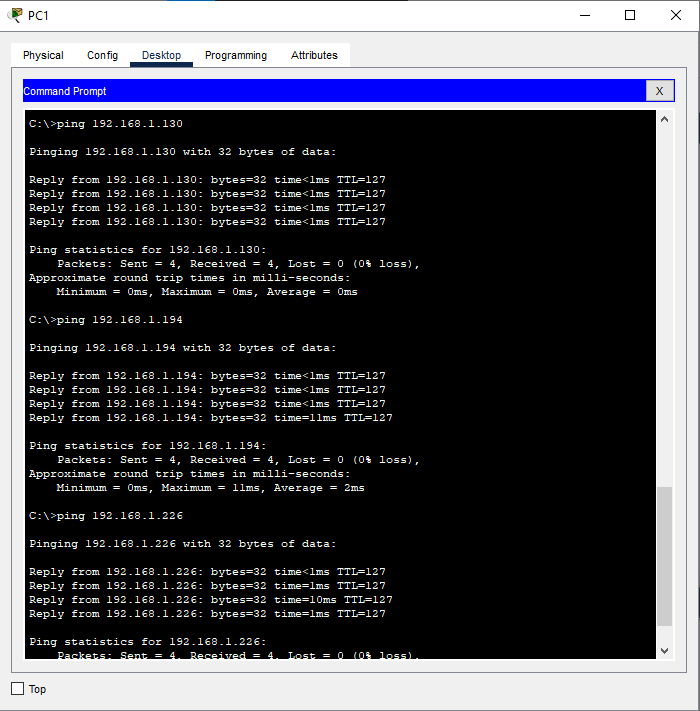
\includegraphics[width=\linewidth]{image/uji ping.png}
      \caption{departemen RnD ke departemen lain}
    \end{subfigure}
    \hspace{1cm}
    \begin{subfigure}[b]{0.3\linewidth}
      \centering
      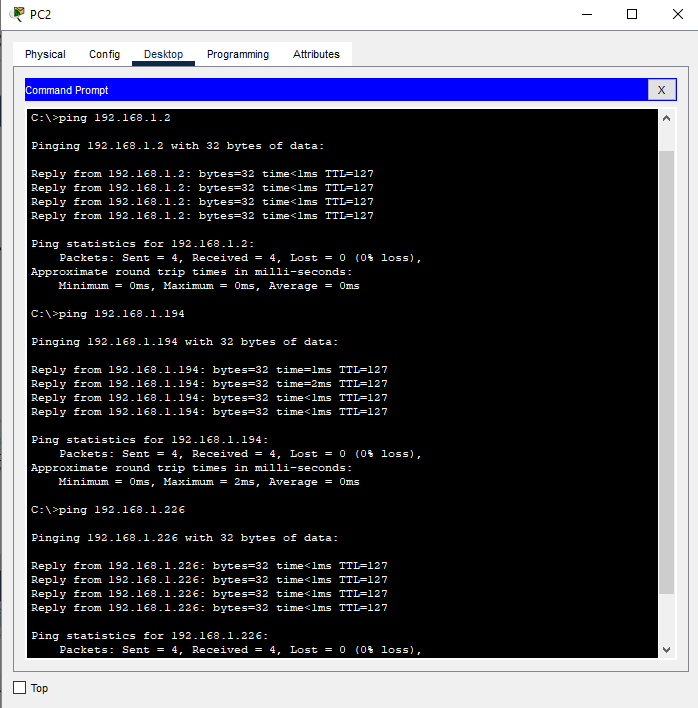
\includegraphics[width=\linewidth]{image/uji ping1.png}
      \caption{departemen produksi ke departemen lain}
    \end{subfigure}
    \hspace{1cm}
    \begin{subfigure}[b]{0.3\linewidth}
      \centering
      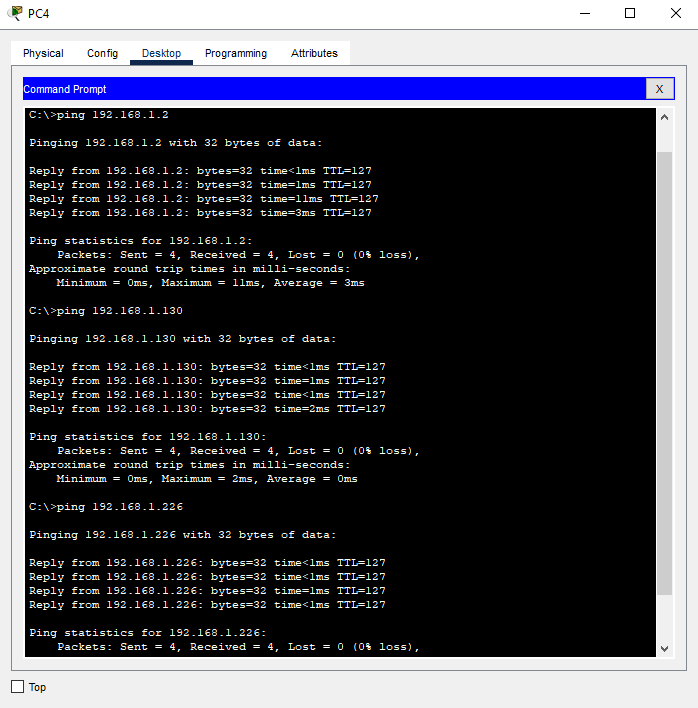
\includegraphics[width=\linewidth]{image/uji ping2.png}
      \caption{departemen administrasi ke departemen lain}
    \end{subfigure}
    \hspace{1cm}
    \begin{subfigure}[b]{0.3\linewidth}
      \centering
      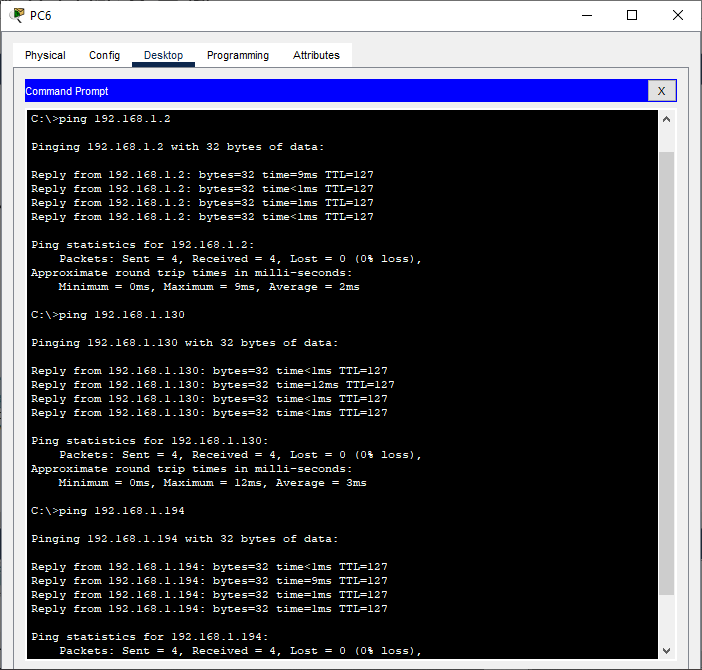
\includegraphics[width=\linewidth]{image/uji ping3.png}
      \caption{departemen keuangan ke departemen lain}
    \end{subfigure}
    \caption{Hasil tes ping pada masing-masing departemen}
\end{figure}

\section{Kesimpulan}
Pada modul 1 ini menjelaskan tentang crimping dan routing yang memberikan pengalaman langsung kepada praktikan dalam membangun konektivitas jaringan komputer menggunakan kabel dan konfigurasi alamat IP menggunakan mikrotik. Tujuan praktikum modul 1 ini adalah untuk memahami dan menerapkan proses pembuatan kabel jaringan menggunakan standar T568A dan memahami konsep dasar IPv4, pengalamatan IP, subnetting, serta implementasi routing sederhana menggunakan IP statis dan dinamis. Hasil percobaan menunjukkan kesesuaian dengan teori jaringan komputer. Kabel yang dikrimping dengan benar berhasil menghubungkan perangkat secara fisik, dan konfigurasi alamat IP serta routing mendukung komunikasi antar perangkat melalui pengujian ping. 

\section{Lampiran}
\subsection{Dokumentasi saat praktikum}
\begin{figure}[H]
    \centering
    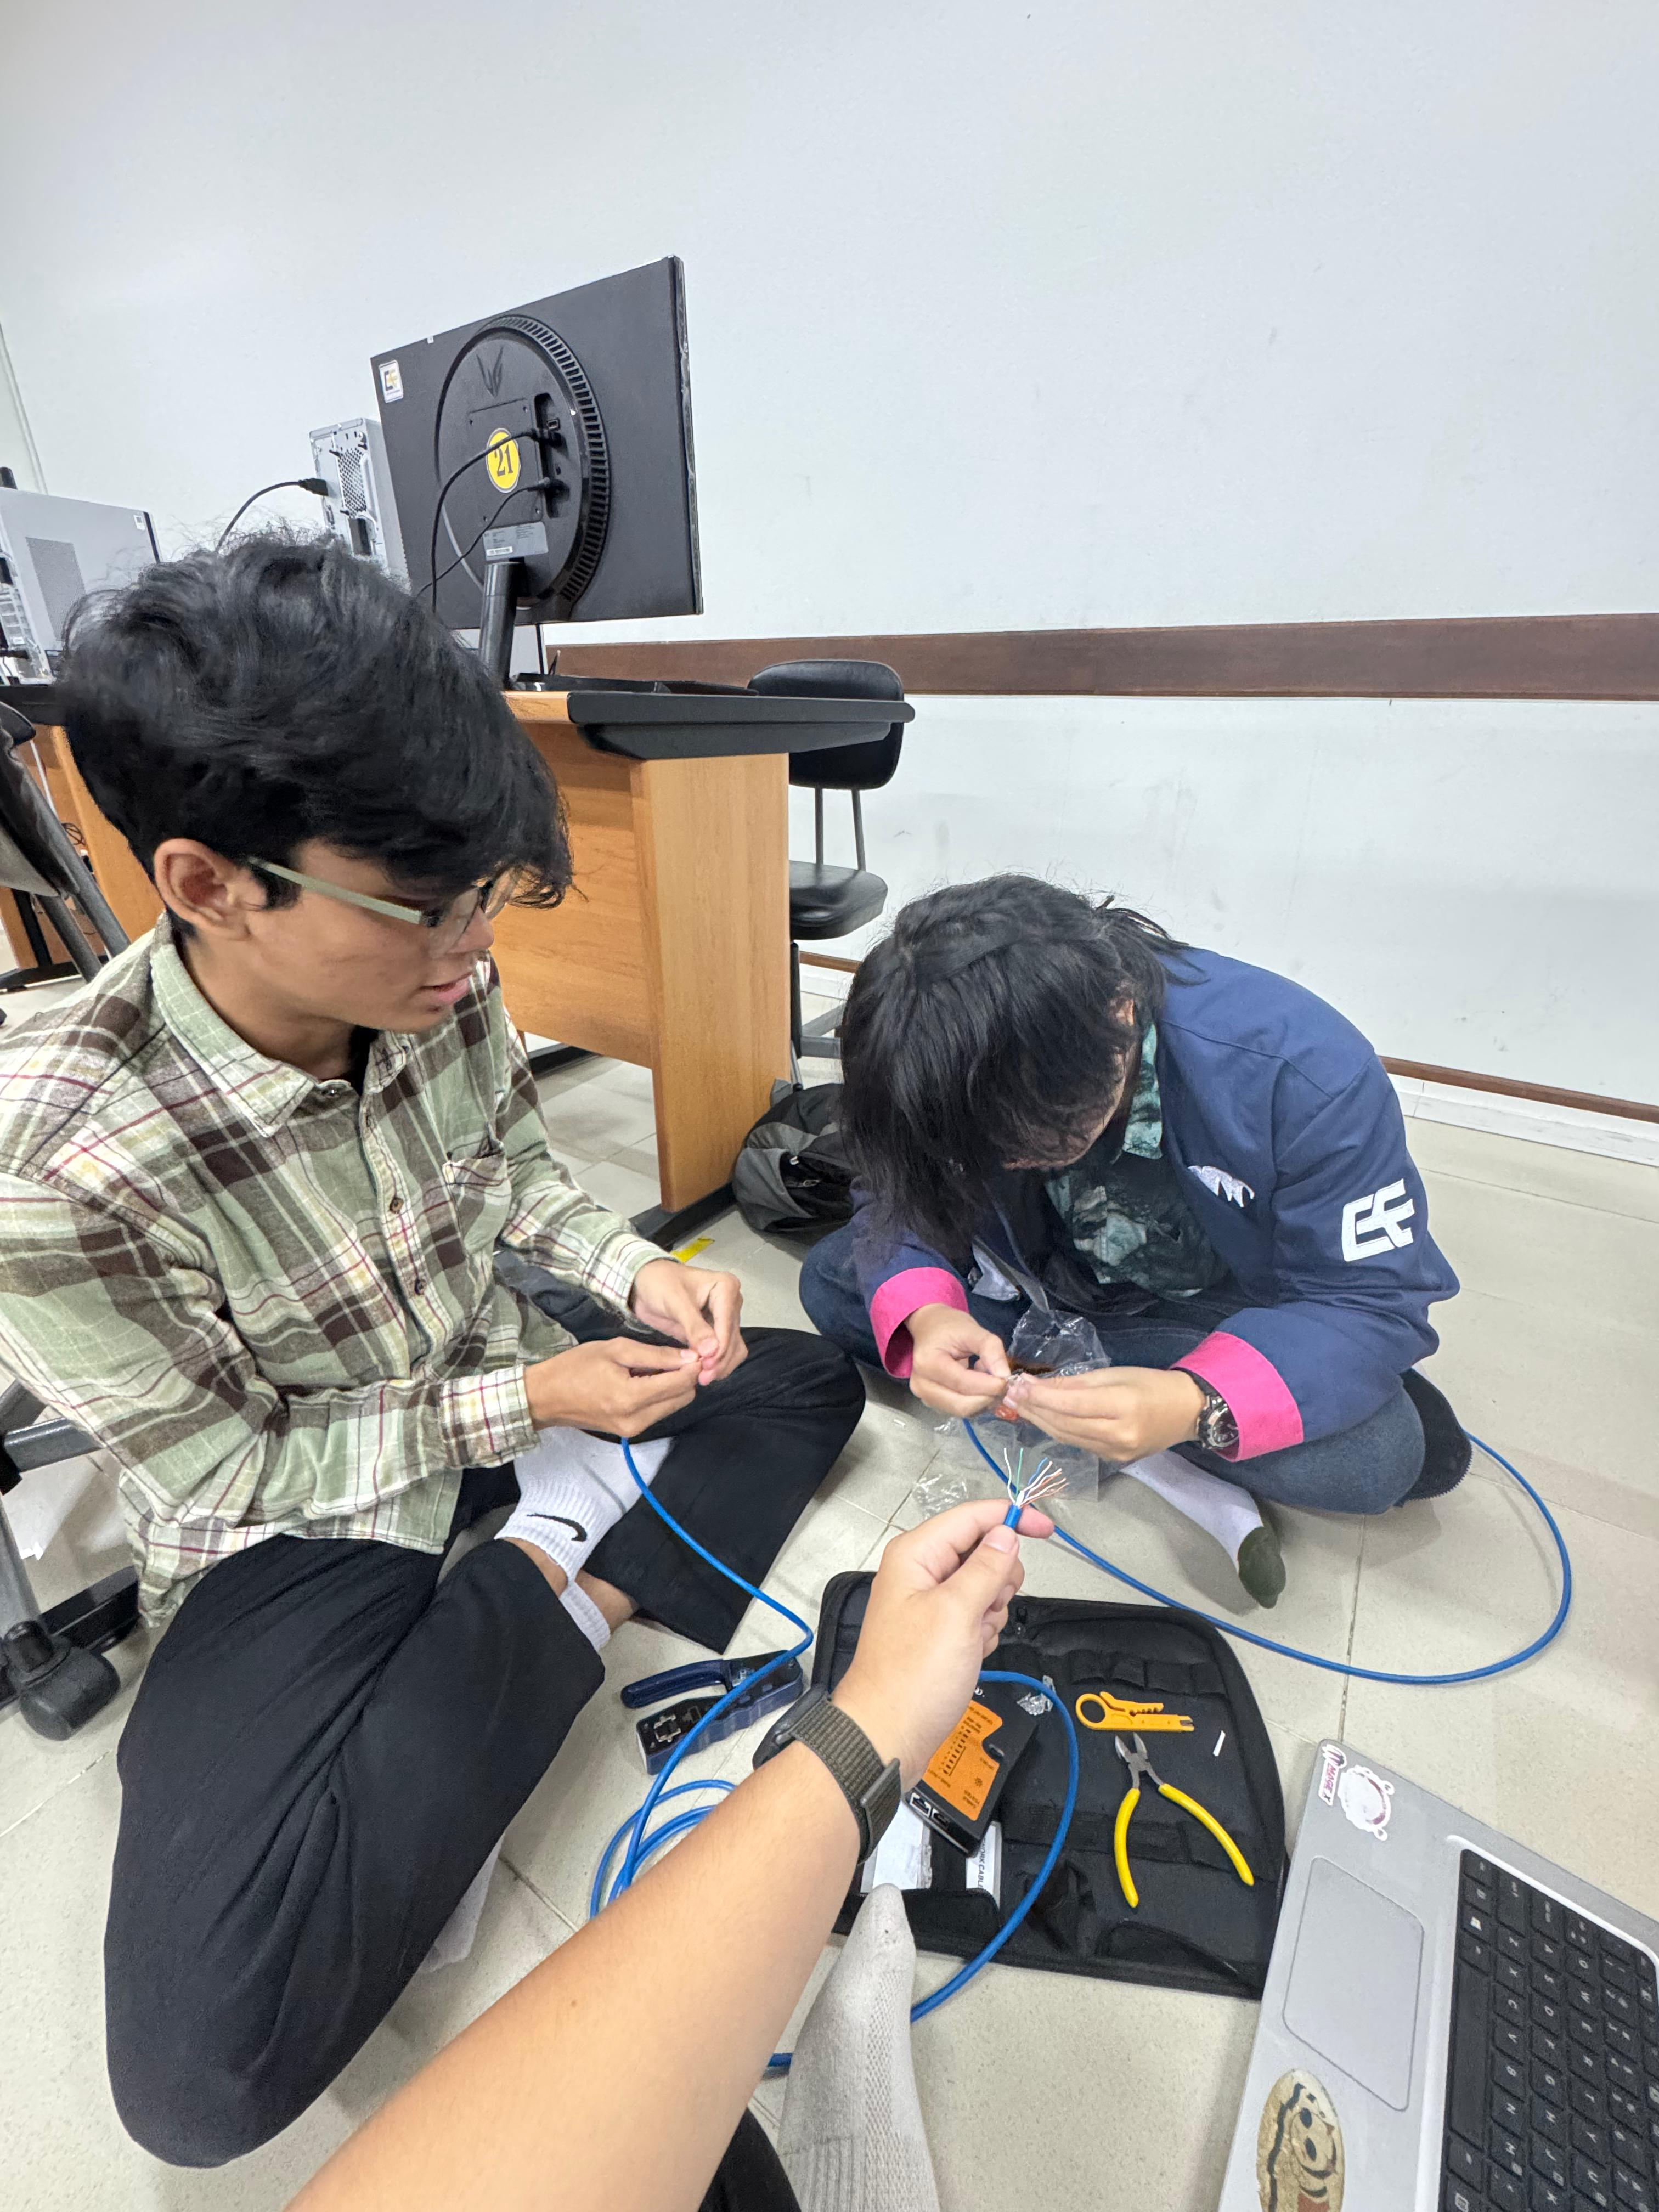
\includegraphics[width=0.65\linewidth]{image/crimping1.jpg}
    \label{fig:inirujukan}
\end{figure}
\begin{figure}[H]
    \centering
    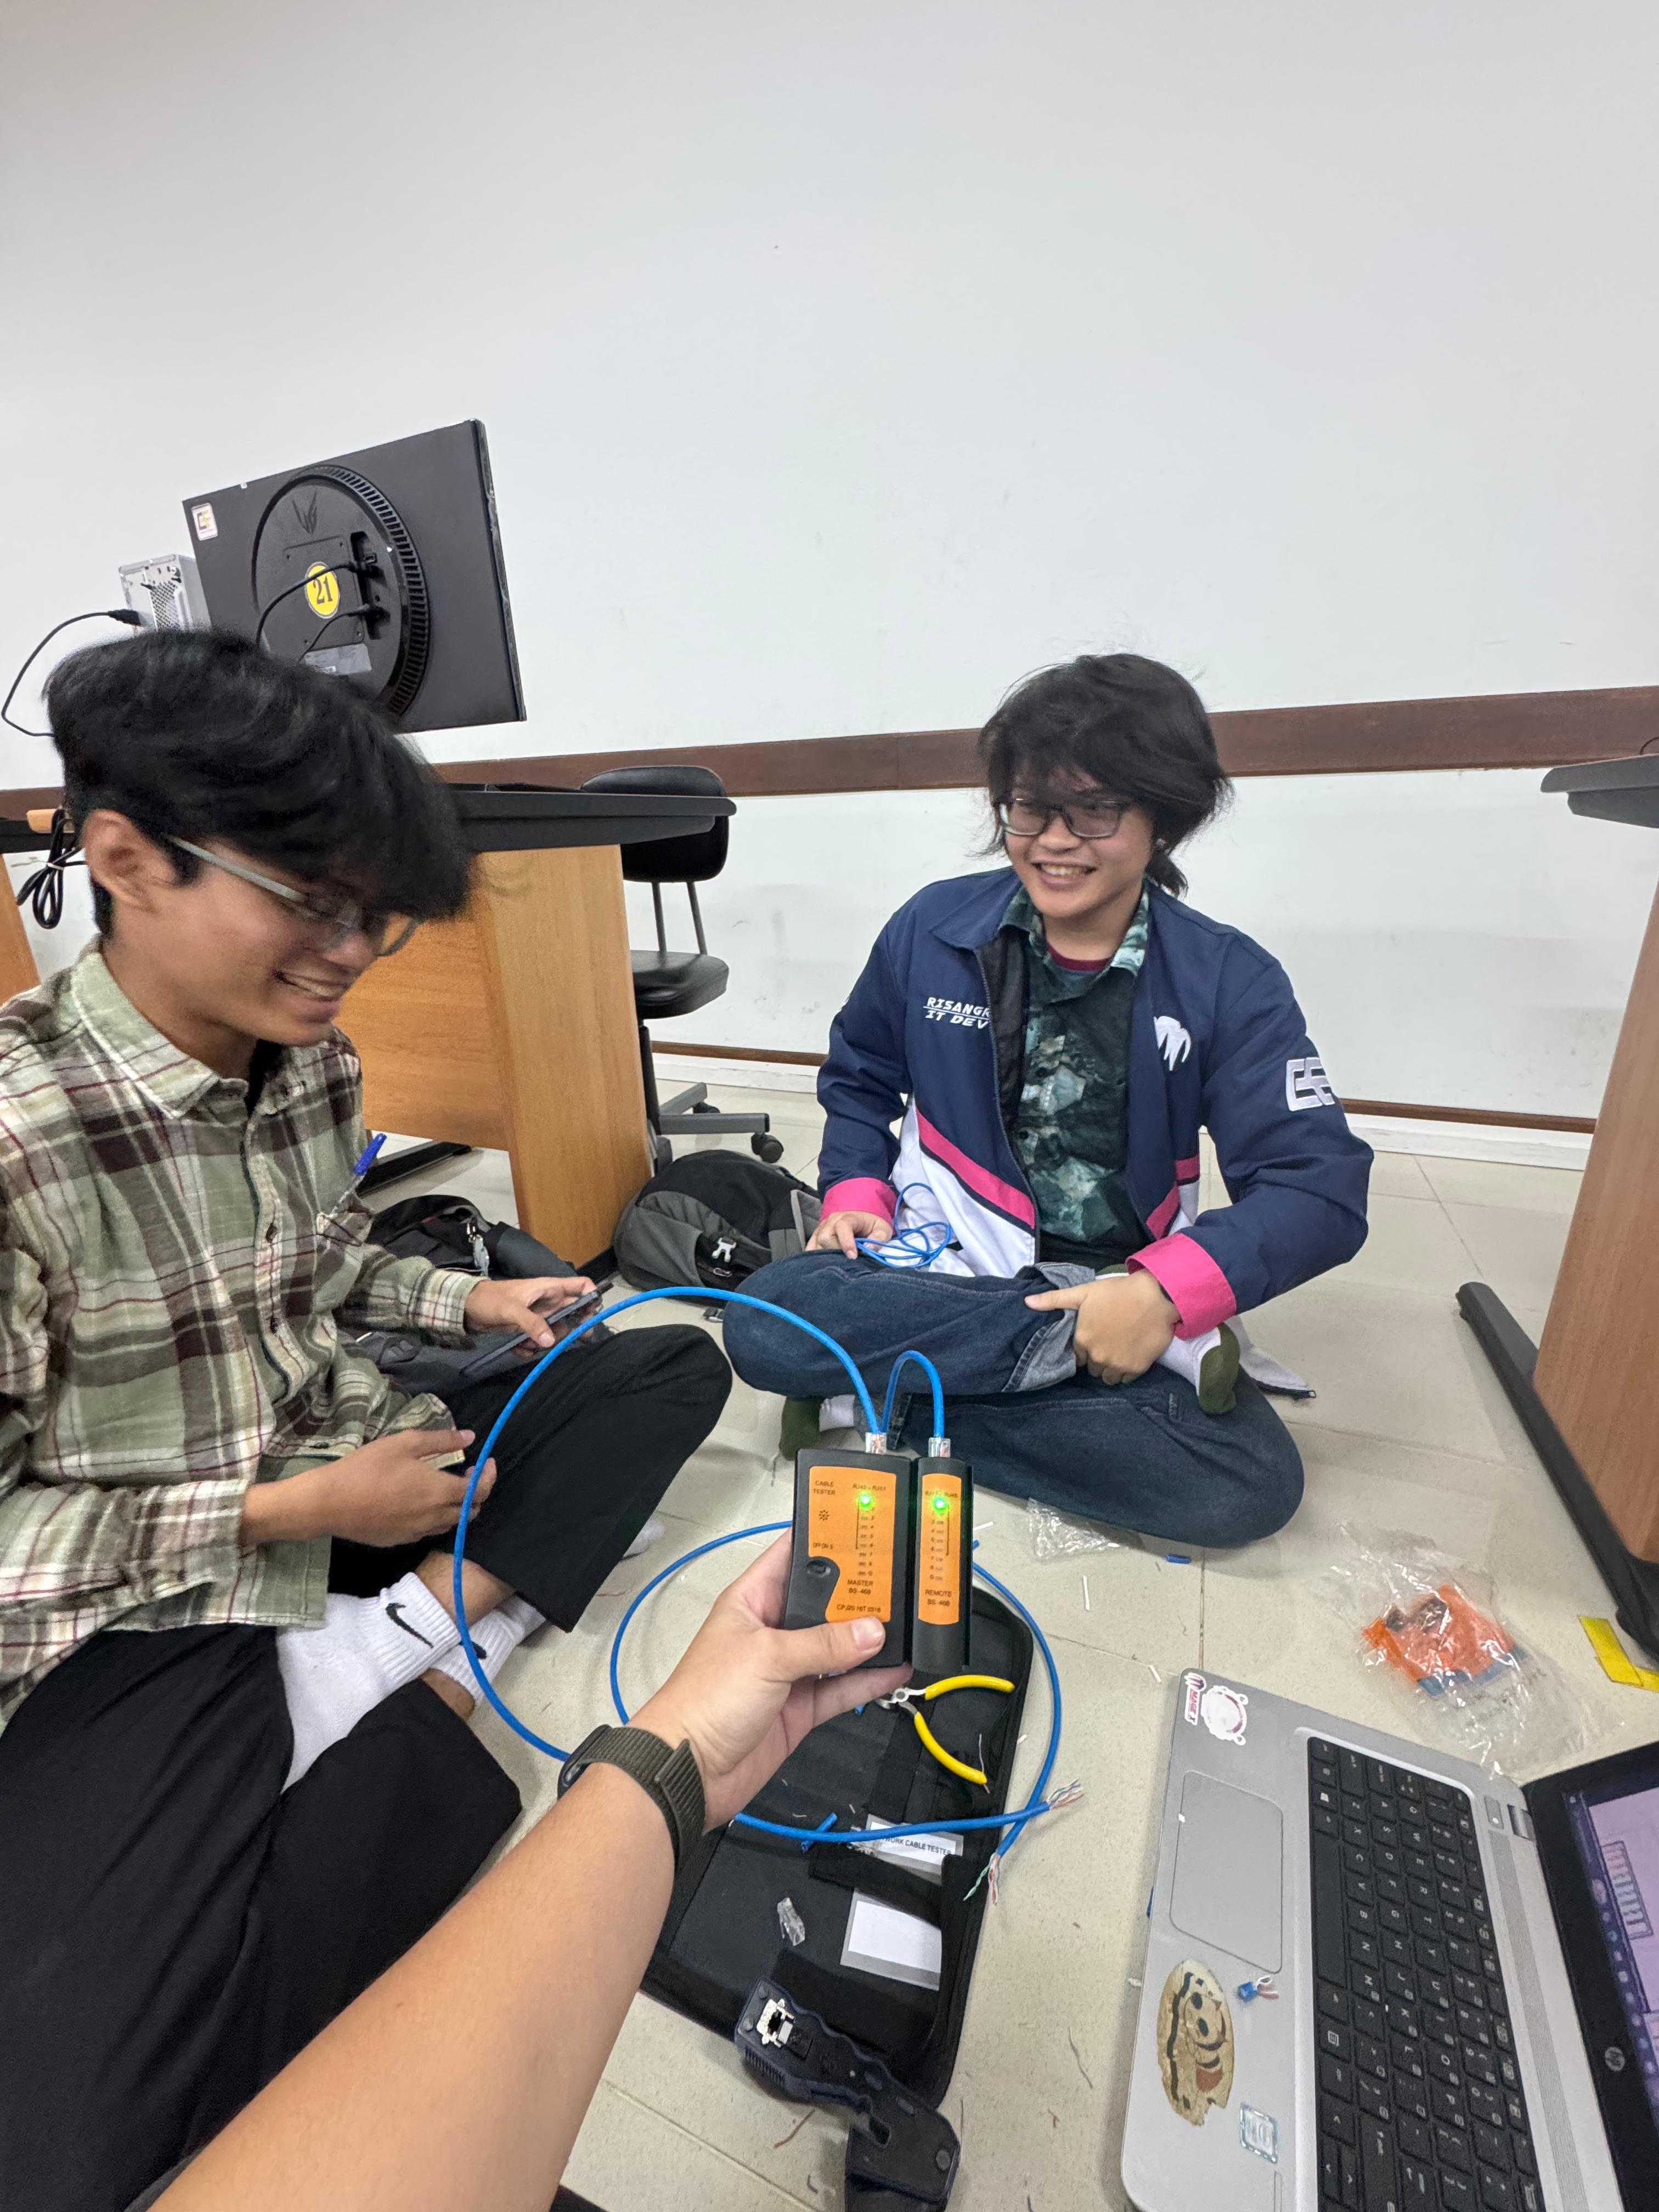
\includegraphics[width=0.65\linewidth]{image/crimping2.jpg}
    \label{fig:inirujukan}
\end{figure}
